% running.tex
%
% This is the `Running SCIRun' main section.

%begin{latexonly}
  \newcommand{\srwindow}%
  {\centerline{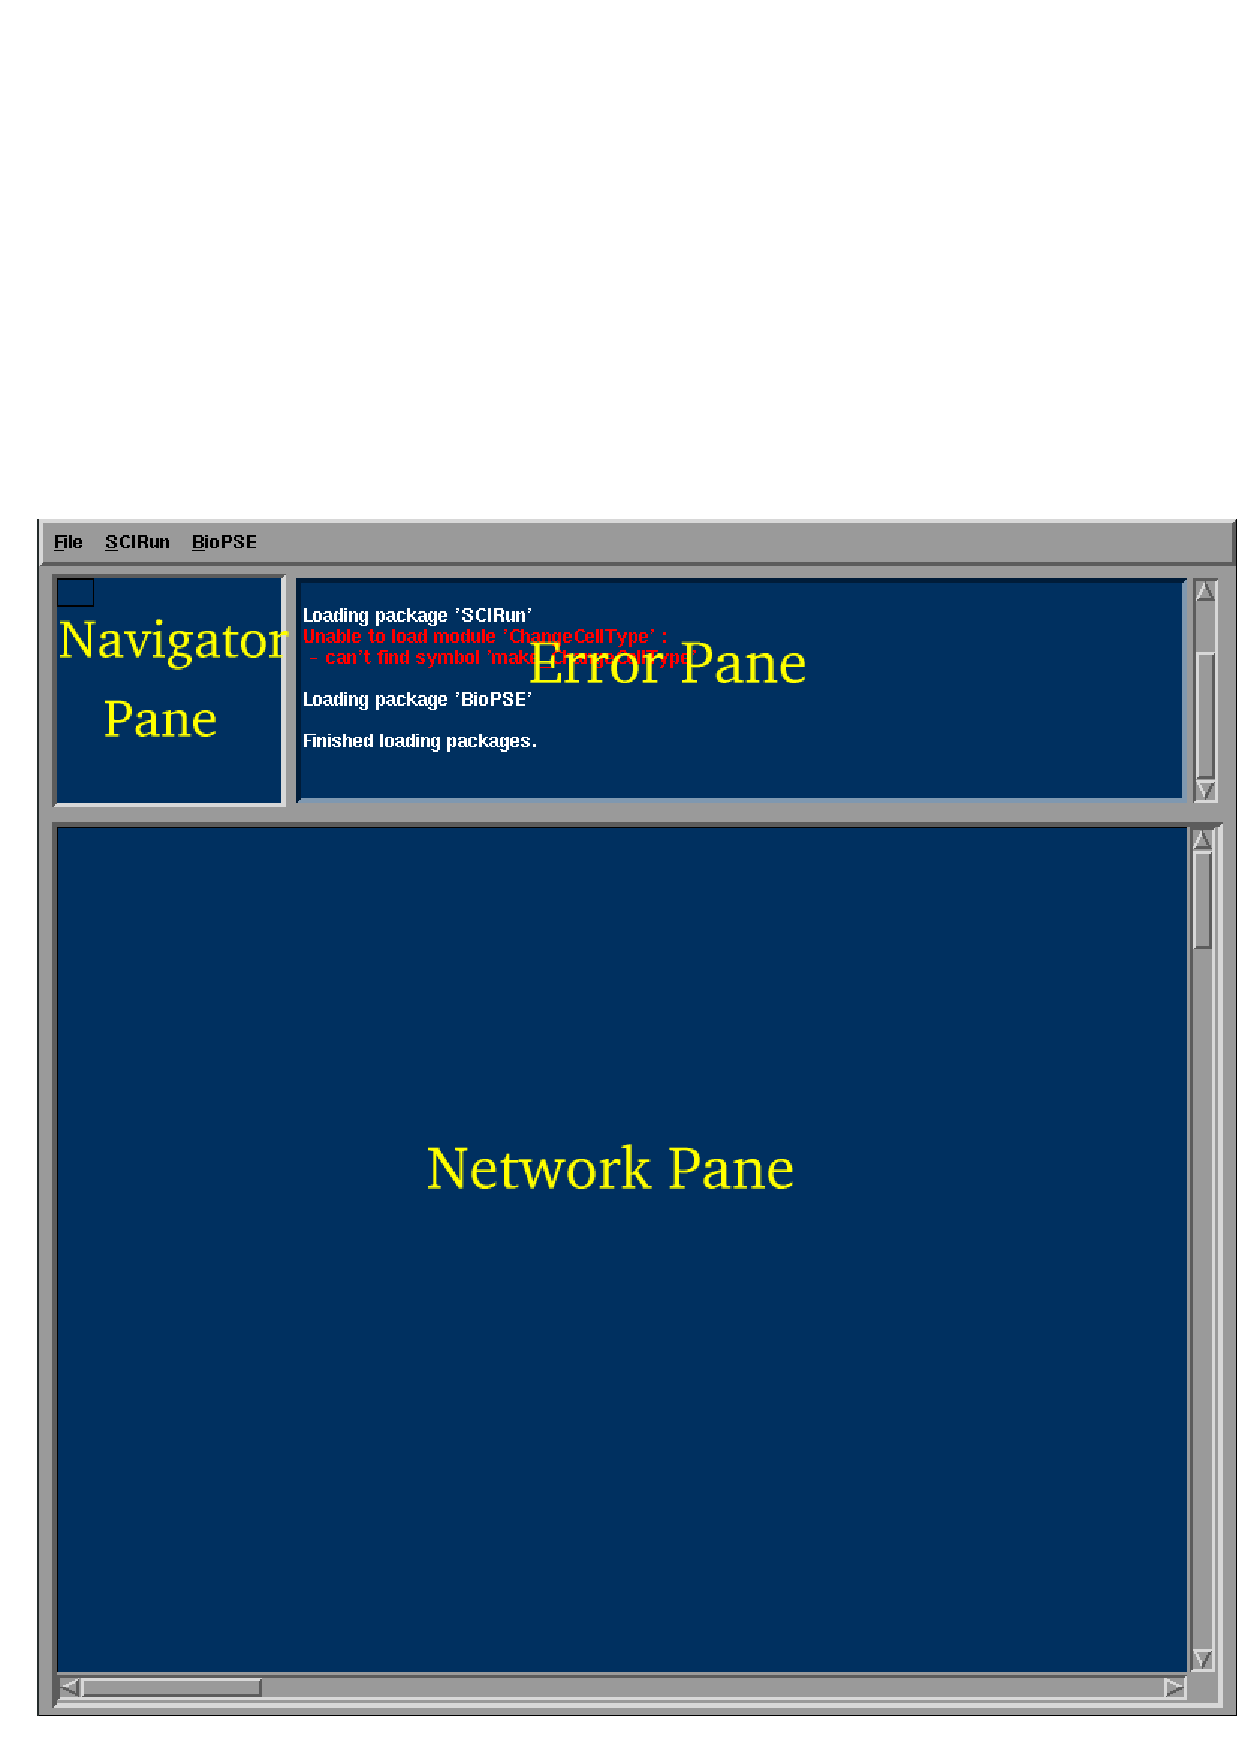
\epsfig{file=Figures/srwindow-1.eps.gz, width=6in,
        bbllx=0, bblly=0, bburx=579, bbury=578}}}
%end{latexonly}
\begin{htmlonly}
  \newcommand{\srwindow}{%
  \htmladdimg[align=top,alt="SCIRun Window"]
  {../Figures/srwindow-1.jpg}}
\end{htmlonly}


\section{Starting \sr{}}
\label{sec:startingup}

\subsection{The \command{scirun} Command}
\label{sec:sciruncmd}

Start \sr{} by typing \keyboard{scirun} in a terminal (\eg \command{xterm})
window.  \note{Don't start \sr{} in the background, \ie don't type
\keyboard{scirun \&}}.

The \command{scirun} command is located in the
\directory{src} directory of the \directory{\sr} install directory.  The
person who installed \sr{} can locate this command for you.


\begin{figure}[htb]
  \begin{makeimage}
  \end{makeimage}
  \srwindow
  \caption{\label{fig:srwindow} \sr{} Main Window}
\end{figure}


Typing \keyboard{scirun} with no arguments starts up \sr{} with a blank \sr{}
window as shown in Figure~\ref{fig:srwindow}.  The main features of this
window are discussed in \secref{Anatomy of the Main
  Window}{sec:windowanatomy}.

The \command{scirun} command may take 1 argument
which is the name of a \sr{} \dfn{network} \index{network} file (these
files have a \filename{.net} extension).  These files hold previously
defined \sr{} networks.  \sr{} will load the specified network.  Network
files will be discussed in a later section.

\sr{} may encounter errors during start up.  These will be displayed in
\sr{}'s error message pane (see Figure~\ref{fig:srwindow}).  These errors
should be \htmladdnormallink{reported}{\bugsurl} to the \sr{} development
team.  \latexonly{See \secref{Reporting Bugs}{sec:bugs} for information on
  reporting bugs.}

\subsection{Anatomy of the Main Window}
\label{sec:windowanatomy}

The \sr{} main window consists of 4 main components (see
Figure~\ref{fig:srwindow}): 

\begin{description}
\item[Menu Bar] The menu bar is used to load networks, save networks, quit
  \sr, create network modules, and perform other tasks.  The menu bar
  consists of the following menu items:

  \begin{description}
  \item[\menu{File}] The \menu{File} menu contains the following items:
    \begin{description}
    \item[Save] Saves the current network to a file.
    \item[Load] Loads a network from a file.
    \item[New] This sub-menu contains items of interest to developers only.
    \item[Add Info] Use this item to add network specific notes to
      the current network.  Notes should be used to document the purpose of
      the network.
    \item[Quit] Quits \sr.
    \end{description}
  \end{description}
  
  \begin{description}
  \item[\menu{SCIRun}] The \menu{SCIRun} menu is used to create modules
    (from the \sr{} package) for use in the network pane.  This menu is
    composed of sub-menus. Each sub-menu corresponds to a \dfn{category}
    \index{category} within the \sr{} package.  A category is a group of
    related modules.  Each menu item in a category sub-menu creates a
    specific module and places it in the network pane.  The network pane's
    pop-up menu (activated by clicking the right most mouse button when the
    mouse pointer is in the network pane) also provides access to the
    \menu{\sr{}} and \menu{\pse{}} (and possibly other) package menus.  An
    overview of the contents of the \sr{} package is given in \secref{The
      \pse{} Package}{sec:biopsepackage}.
  \end{description}

  \begin{description}
  \item[\menu{BioPSE}] The \menu{BioPSE} menu is used to create modules
    (from the \pse package) for use in the network pane.  It consists
    of category sub-menus and module menu items.   An overview of the
    contents of the \sr{} package is given in \secref{The SCIRun
      Package}{sec:srpackage}.
  \end{description}

  \begin{description}
  \item [\textit{Other Package Menus}] There may be other package
    menus if other packages have been installed.  They too will consist
    of category sub-menus and module menu items.
  \end{description}
  
\item[Navigator Pane] The Navigator Pane is located in the upper left
  corner of the main window (see Figure~\ref{fig:srwindow}). It is used to
  navigate complex networks.  The use of the Navigator Pane will be
  described in \secref{Navigating a Network}{sec:navnetwork}.
  
\item[Error Pane] Errors during program startup are displayed in the Error
  Pane.  It is located in the upper right corner of the main window(see
  Figure~\ref{fig:srwindow}).  Errors on startup may mean that \sr{} has
  been installed incorrectly or has been installed from a buggy
  distribution.  Please \hyperref{report}{(see Section~}{)}{sec:bugs} these
  errors.
  
\item[Network Pane] The Network Pane occupies the bottom of the main
  window(see Figure~\ref{fig:srwindow}).  It is used to build and execute
  networks.  \secref{Building Networks}{sec:workwithnets} discusses the use
  of this pane.

\end{description}

\subsection{The Terminal Window}
\label{sec:termwinapp}

After starting, \sr{} will also run a shell-like application in the
terminal window called the \dfn{\sr{} shell}.  The \sr{} shell displays the
prompt \screen{scirun\ra}.  This program is actually a modified \dfna{Tool
  Command Language}{TCL} shell program and it is possible to type in
\acronym{TCL}'ish \sr{} commands at the prompt. The use of this program
will be described in \hyperref{a later section}{Section~}{}{sec:termapp}.


\subsection{Environment Variables}
\label{sec:environ} 
\index{Environment Variables}

There are several environment variables that \sr{} uses to make it easier
to use.  These are all optional, but paying attention to them can make it
easier to find files during a \sr{} session and to improve performance via
remote connections.

\begin{description}
  \item{\envvar{SCIRUN\_DATA}}\mbox{}: ]
        \index{SCIRUN\_DATA}
        \label{sec:scirundata}
        The environment variable \envvar{SCIRUN\_DATA} specifies the
        default directory of \sr{} data files.  \sr will first look in this
        directory to find data and network files.  It affects the behavior
        of file browsing dialogs -- they will prompt for a file within the
        \envvar{SCIRUN\_DATA} directory (of course you may have the dialog
        look elsewhere).  This can be very handy when using shared
        datasets, like the one shipped with the software.  Many of the
        demonstration nets with the software also assume that
        \envvar{SCIRUN\_DATA} points to the location of these datasets.

  \item[\envvar{SCIRUN\_DATASET}\mbox{}: ]\mbox{}
        \label{sec:scirundataset} 
        This variable refines the search for data files within the director
        pointed at by \envvar{SCIRUN\_DATA}.  By setting these two
        variables, one can easily select different data sets for the same
        network.  See the network files distributed with the software, for
        example \filename{forward-fem.net}, so examples of how to use these
        variables.  Some of the demonstration nets do require setting
        \envvar{SCIRUN\_DATASET} so see the documentation on those.

      \item[\envvar{DISPLAY}: ]\mbox{}
        
        If \sr is executed remotely then the value of the \envvar{DISPLAY}
        variable (as set on the remote machine) must be set correctly and
        the remote machine must be allowed to talk to the local X11 server.
        
        For telnet-like (unencrypted) connections to a remote machine you
        may set \envvar{DISPLAY} as follows:

\begin{verbatim}
  export DISPLAY=local-ip-addres:0.0
\end{verbatim}
        
        for an sh-style shell. And like this:

\begin{verbatim}
setenv DISPLAY local-ip-addres:0.0
\end{verbatim}

        for a csh-style shell.

        When connecting to a remote machine using ssh, \envvar{DISPLAY} is
        normally set automatically (depending on how ssh has been
        configured).  This results in poor display performance however
        because of encryption activity on the connection.  To increase
        performance you may override the value of \envvar{DISPLAY} provided
        by ssh.  Simply set \envvar{DISPLAY} as
        shown above.  Note that this technique defeats the encryption
        protection on the X11 connection.

        You will need to grant the remote machine permission to display on
        your local machine if you are using a telnet-like connection or if
        you are overriding the value of \envvar{DISPLAY} provided by ssh.
        Use the \command{xhost} command on the local machine to do this:

\begin{verbatim}
xhost +remote-machine-name
\end{verbatim}

\end{description}



\subsection{Quitting or Exiting \sr{}}
\label{sec:stopping}

Quit \sr{} by selecting the \menuitem{Quit} item from the \menu{File} menu

\warning{Don't press \keyboard{control-c} to exit \sr.  Doing this will
drop you into a debugger which is probably not what you want to do}.


%%% Local Variables: 
%%% mode: latex
%%% TeX-master: "usersguide"
%%% End: 
